
% TODO - remove areas of interest
%      - maybe add section - what is important for me
%      - add highlight section project items
%      - add links google play web pages of employers
%
%
%




%-----------------------------------------------------------------------------------------------------------------------------------------------%
%	The MIT License (MIT)
%
%	Copyright (c) 2016 Jan Küster
%
%	Permission is hereby granted, free of charge, to any person obtaining a copy
%	of this software and associated documentation files (the "Software"), to deal
%	in the Software without restriction, including without limitation the rights
%	to use, copy, modify, merge, publish, distribute, sublicense, and/or sell
%	copies of the Software, and to permit persons to whom the Software is
%	furnished to do so, subject to the following conditions:
%	
%	THE SOFTWARE IS PROVIDED "AS IS", WITHOUT WARRANTY OF ANY KIND, EXPRESS OR
%	IMPLIED, INCLUDING BUT NOT LIMITED TO THE WARRANTIES OF MERCHANTABILITY,
%	FITNESS FOR A PARTICULAR PURPOSE AND NONINFRINGEMENT. IN NO EVENT SHALL THE
%	AUTHORS OR COPYRIGHT HOLDERS BE LIABLE FOR ANY CLAIM, DAMAGES OR OTHER
%	LIABILITY, WHETHER IN AN ACTION OF CONTRACT, TORT OR OTHERWISE, ARISING FROM,
%	OUT OF OR IN CONNECTION WITH THE SOFTWARE OR THE USE OR OTHER DEALINGS IN
%	THE SOFTWARE.
%
%	*************	RESOURCES USED	 ********************
%
%	http://tex.stackexchange.com/questions/5718/package-for-pie-charts
%	http://tex.stackexchange.com/questions/183087/draw-colored-world-us-map-in-latex#183138
%	http://www.texample.net/tikz/examples/simple-flow-chart/
%	http://vizualize.me/#
%	http://devnet.kentico.com/getattachment/fd511a92-e164-40f5-ba51-07c228a49fed/Kentico_fortune500_infographics_FINAL.png
%
%-----------------------------------------------------------------------------------------------------------------------------------------------%


%============================================================================%
%
%	DOCUMENT DEFINITION
%
%============================================================================%

%we use article class because we want to fully customize the page
\documentclass[10pt,A4]{article}	


%----------------------------------------------------------------------------------------
%	ENCODING
%----------------------------------------------------------------------------------------

%we use utf8 since we want to build from any machine
\usepackage[utf8]{inputenc}		

%----------------------------------------------------------------------------------------
%	LOGIC
%----------------------------------------------------------------------------------------

\usepackage{xifthen}
\usepackage{calc}

%----------------------------------------------------------------------------------------
%	FONT
%----------------------------------------------------------------------------------------

% some tex-live fonts - choose your own

%\usepackage[defaultsans]{droidsans}
%\usepackage[default]{comfortaa}
%\usepackage{cmbright}
\usepackage[default]{raleway}
%\usepackage{fetamont}
%\usepackage[default]{gillius}
%\usepackage[light,math]{iwona}
%\usepackage[thin]{roboto} 

% set font default
\renewcommand*\familydefault{\sfdefault} 	
\usepackage[T1]{fontenc}

% more font size definitions
\usepackage{moresize}		

% awesome font
\usepackage{fontawesome}


%----------------------------------------------------------------------------------------
%	PAGE LAYOUT  DEFINITIONS
%----------------------------------------------------------------------------------------

%debug page outer frames
%\usepackage{showframe}			

%define page styles using geometry
\usepackage[a4paper]{geometry}		

% for example, change the margins to 2 inches all round
\geometry{top=1cm, bottom=1cm, left=1cm, right=1cm} 	

% use customized header
\usepackage{fancyhdr}				
\pagestyle{fancy}

%less space between header and content
\setlength{\headheight}{-5pt}		

% customize header entries
\lhead{}
\rhead{}
\chead{}

%indentation is zero
\setlength{\parindent}{0mm}

%----------------------------------------------------------------------------------------
%	TABLE /ARRAY DEFINITIONS
%---------------------------------------------------------------------------------------- 

%extended aligning of tabular cells
\usepackage{array}

% custom column width
\newcolumntype{x}[1]{%
>{\raggedleft\hspace{0pt}}p{#1}}%


%----------------------------------------------------------------------------------------
%	GRAPHICS DEFINITIONS
%---------------------------------------------------------------------------------------- 

\usepackage{graphicx}
\usepackage{wrapfig}

\usepackage{longtable} % Required for tables that span multiple pages

\usepackage[hidelinks]{hyperref} % Required for links but hide the default boxes around links

% for drawing graphics and charts
\usepackage{tikz}
\usetikzlibrary{shapes, backgrounds}

% use to vertically center content
% credits to: http://tex.stackexchange.com/questions/7219/how-to-vertically-center-two-images-next-to-each-other
\newcommand{\vcenteredinclude}[1]{\begingroup
\setbox0=\hbox{\includegraphics{#1}}%
\parbox{\wd0}{\box0}\endgroup}

% use to vertically center content
% credits to: http://tex.stackexchange.com/questions/7219/how-to-vertically-center-two-images-next-to-each-other
\newcommand*{\vcenteredhbox}[1]{\begingroup
\setbox0=\hbox{#1}\parbox{\wd0}{\box0}\endgroup}

%----------------------------------------------------------------------------------------
%	ICON-SET EMBEDDING
%---------------------------------------------------------------------------------------- 

% at this point we simplify our icon-embedding by simply referring to a set of png images.
% if you find a good way of including svg without conflicting with other packages you can
% replace this part
\newcommand{\icon}[2]{\colorbox{thirdcol}{\makebox(#2, #2){\textcolor{sectcol}{\csname fa#1\endcsname}}}}	%icon shortcut
\newcommand{\icontext}[3]{ 						%icon with text shortcut
	\vcenteredhbox{\icon{#1}{#2}} \vcenteredhbox{\textcolor{textcol}{#3}}
}

%----------------------------------------------------------------------------------------
%	Color DEFINITIONS
%---------------------------------------------------------------------------------------- 

\usepackage{xcolor}

%defineColors
\definecolor{orange}{RGB}{255,150,0}
\definecolor{lblue}{RGB}{0,178,255}
\definecolor{darkblue}{RGB}{0,80,130}
\definecolor{darkerblue}{RGB}{0,100,160}
\definecolor{lgray}{RGB}{0,120,200}
\definecolor{powderblue}{RGB}{190,220,255}
\definecolor{darkestblue}{RGB}{0,50,80}


%main color
\colorlet{maincol}{orange}

%secondary colors
\colorlet{secondcol}{lblue}
\colorlet{thirdcol}{darkblue}
\colorlet{fourthcol}{darkerblue}
\colorlet{fifthcol}{lgray}
\colorlet{sixthcol}{darkblue}

%background color
\colorlet{bgcol}{powderblue}

%textcolor
\colorlet{textcol}{darkestblue}

%titletextcolor
\colorlet{titletext}{white}

%sectioncolor
\colorlet{sectcol}{white}

%set a background col for whole page
\pagecolor{bgcol}


%----------------------------------------------------------------------------------------
% 	HEADER
%----------------------------------------------------------------------------------------

% remove top header line
\renewcommand{\headrulewidth}{0pt} 

%remove botttom header line
\renewcommand{\footrulewidth}{0pt}	  	

%remove pagenum
\renewcommand{\thepage}{}	

%remove section num		
\renewcommand{\thesection}{}			


%----------------------------------------------------------------------------------------
%
% 	TIKZ GRAPHICS
%
%----------------------------------------------------------------------------------------


% the chart graphics are outsourced into own files

%----------------------------------------------------------------------------------------
% 	PIE CHART
%----------------------------------------------------------------------------------------
%-----------------------------------------------------------------------------------------------------------------------------------------------%
%	The MIT License (MIT)
%
%	Copyright (c) 2016 Jan Küster
%
%	Permission is hereby granted, free of charge, to any person obtaining a copy
%	of this software and associated documentation files (the "Software"), to deal
%	in the Software without restriction, including without limitation the rights
%	to use, copy, modify, merge, publish, distribute, sublicense, and/or sell
%	copies of the Software, and to permit persons to whom the Software is
%	furnished to do so, subject to the following conditions:
%	
%	THE SOFTWARE IS PROVIDED "AS IS", WITHOUT WARRANTY OF ANY KIND, EXPRESS OR
%	IMPLIED, INCLUDING BUT NOT LIMITED TO THE WARRANTIES OF MERCHANTABILITY,
%	FITNESS FOR A PARTICULAR PURPOSE AND NONINFRINGEMENT. IN NO EVENT SHALL THE
%	AUTHORS OR COPYRIGHT HOLDERS BE LIABLE FOR ANY CLAIM, DAMAGES OR OTHER
%	LIABILITY, WHETHER IN AN ACTION OF CONTRACT, TORT OR OTHERWISE, ARISING FROM,
%	OUT OF OR IN CONNECTION WITH THE SOFTWARE OR THE USE OR OTHER DEALINGS IN
%	THE SOFTWARE.
%
%-----------------------------------------------------------------------------------------------------------------------------------------------%

%counters for chart loop
\newcounter{a}
\newcounter{b}
\newcounter{c}

% draw a slice for a chart
% param 1: Circle form - 90 = quarter, 180 = half, 360 = full
% param 2: scale default=1 (scales only chart, not label text)
% param 3: border color
% param 4: label text color
% param 5: label bg color
% param 6:
\newenvironment{piechart}[5] {

	% draw a slice for a chart
	% param 1: value x of 100
	% param 2: label text
	% param 3: fill color
	% param 4:
	% param 5:
	% param 6:
	\newcommand{\slice}[3] {

		\setcounter{a}{\value{b}}
		\addtocounter{b}{##1}

		%set from angle point
		\pgfmathparse{\thea/100*#1}
	  	\let\pointa\pgfmathresult

		%set toanglepoint
		\pgfmathparse{\theb/100*#1}
	  	\let\pointb\pgfmathresult

		%set midangle
	 	\pgfmathparse{0.5*\pointa+0.5*\pointb}
	  	\let\midangle\pgfmathresult
		
		% draw the slice
	  	\filldraw[fill=##3!100,draw=#3!100, line width=2pt ] (0,0) -- (\pointa:#2) arc (\pointa:\pointb:#2) -- cycle;

	  	% draw label
	  	\node[label=\midangle:\colorbox{#5}{\textcolor{#4}{##2}}] at (\midangle:#2) {};

		\filldraw[fill=#3,draw=none] (0,0) circle (#2/2);
	}

	% execute commands
	\setcounter{a}{0}
	\setcounter{b}{0}
	\begin{tikzpicture}
}
{\end{tikzpicture}}

%----------------------------------------------------------------------------------------
% 	BAR CHART
%----------------------------------------------------------------------------------------
%-----------------------------------------------------------------------------------------------------------------------------------------------%
%	The MIT License (MIT)
%
%	Copyright (c) 2016 Jan Küster
%
%	Permission is hereby granted, free of charge, to any person obtaining a copy
%	of this software and associated documentation files (the "Software"), to deal
%	in the Software without restriction, including without limitation the rights
%	to use, copy, modify, merge, publish, distribute, sublicense, and/or sell
%	copies of the Software, and to permit persons to whom the Software is
%	furnished to do so, subject to the following conditions:
%	
%	THE SOFTWARE IS PROVIDED "AS IS", WITHOUT WARRANTY OF ANY KIND, EXPRESS OR
%	IMPLIED, INCLUDING BUT NOT LIMITED TO THE WARRANTIES OF MERCHANTABILITY,
%	FITNESS FOR A PARTICULAR PURPOSE AND NONINFRINGEMENT. IN NO EVENT SHALL THE
%	AUTHORS OR COPYRIGHT HOLDERS BE LIABLE FOR ANY CLAIM, DAMAGES OR OTHER
%	LIABILITY, WHETHER IN AN ACTION OF CONTRACT, TORT OR OTHERWISE, ARISING FROM,
%	OUT OF OR IN CONNECTION WITH THE SOFTWARE OR THE USE OR OTHER DEALINGS IN
%	THE SOFTWARE.
%
%-----------------------------------------------------------------------------------------------------------------------------------------------%
\newcounter{barcount}


% draw a bar chart
% param 1: width
% param 2: height
% param 3: border color
% param 4: label text color
% param 5: label bg color
% param 6: cat 1 color
\newenvironment{barchart}[8]{

	\newcommand{\barwidth}{0.35}
	\newcommand{\barsep}{0.2}

	% param 1: overall percent
	% param 2: label
	% param 3: cat 1 percent
	% param 4: cat 2 percent
	% param 5: cat 3 percent
	\newcommand{\baritem}[5]{

		\pgfmathparse{##3+##4+##5}
		 \let\perc\pgfmathresult

		\pgfmathparse{#2}
		 \let\barsize\pgfmathresult
	
		\pgfmathparse{\barsize*##3/100}
		 \let\barone\pgfmathresult
	
		\pgfmathparse{\barsize*##4/100}
		 \let\bartwo\pgfmathresult
	
		\pgfmathparse{\barsize*##5/100}
		 \let\barthree\pgfmathresult

		\pgfmathparse{(\barwidth*\thebarcount)+(\barsep*\thebarcount)}
		 \let\barx\pgfmathresult

		\filldraw[fill=#6, draw=none] (0,-\barx) rectangle (\barone,-\barx-\barwidth);
		\filldraw[fill=#7, draw=none] (\barone, -\barx) rectangle (\barone+\bartwo,-\barx-\barwidth);
		\filldraw[fill=#8, draw=none] (\barone+\bartwo,-\barx ) rectangle (\barone+\bartwo+\barthree,-\barx-\barwidth);

		\node [label=180:\colorbox{#5}{\textcolor{#4}{##2}}] at (0,-\barx-0.175) {};
		\addtocounter{barcount}{1}
	}
	\begin{tikzpicture}
	\setcounter{barcount}{0}
	
}
{\end{tikzpicture}}


%----------------------------------------------------------------------------------------
% 	BUBBLE CHART
%----------------------------------------------------------------------------------------
%-----------------------------------------------------------------------------------------------------------------------------------------------%
%	The MIT License (MIT)
%
%	Copyright (c) 2016 Jan Küster
%
%	Permission is hereby granted, free of charge, to any person obtaining a copy
%	of this software and associated documentation files (the "Software"), to deal
%	in the Software without restriction, including without limitation the rights
%	to use, copy, modify, merge, publish, distribute, sublicense, and/or sell
%	copies of the Software, and to permit persons to whom the Software is
%	furnished to do so, subject to the following conditions:
%	
%	THE SOFTWARE IS PROVIDED "AS IS", WITHOUT WARRANTY OF ANY KIND, EXPRESS OR
%	IMPLIED, INCLUDING BUT NOT LIMITED TO THE WARRANTIES OF MERCHANTABILITY,
%	FITNESS FOR A PARTICULAR PURPOSE AND NONINFRINGEMENT. IN NO EVENT SHALL THE
%	AUTHORS OR COPYRIGHT HOLDERS BE LIABLE FOR ANY CLAIM, DAMAGES OR OTHER
%	LIABILITY, WHETHER IN AN ACTION OF CONTRACT, TORT OR OTHERWISE, ARISING FROM,
%	OUT OF OR IN CONNECTION WITH THE SOFTWARE OR THE USE OR OTHER DEALINGS IN
%	THE SOFTWARE.
%
%-----------------------------------------------------------------------------------------------------------------------------------------------%


\newcommand{\bubble}[5]{
	\definecolor{tmpcol}{RGB}{50,50,#5}
	% slice
  	\filldraw[fill=thirdcol,draw=none] (#1,0.5) circle (#3);

  	% outer label
  	\node[label=\textcolor{textcol}{#4}] at (#1,0.7) {};
}

\newcommand{\bubbles}[2]{
	%reset counters
	\setcounter{a}{0}
	\setcounter{c}{150}
	\begin{tikzpicture}[scale=3]
	\foreach \p/\t in {#1} {
	    	\addtocounter{a}{1}
	    	\bubble{\thea/2}{\theb}{\p/25}{\t}{1\p0}
	}
	\end{tikzpicture}
}

%----------------------------------------------------------------------------------------
% 	SQUARE CHART
%----------------------------------------------------------------------------------------
%-----------------------------------------------------------------------------------------------------------------------------------------------%
%	The MIT License (MIT)
%
%	Copyright (c) 2016 Jan Küster
%
%	Permission is hereby granted, free of charge, to any person obtaining a copy
%	of this software and associated documentation files (the "Software"), to deal
%	in the Software without restriction, including without limitation the rights
%	to use, copy, modify, merge, publish, distribute, sublicense, and/or sell
%	copies of the Software, and to permit persons to whom the Software is
%	furnished to do so, subject to the following conditions:
%	
%	THE SOFTWARE IS PROVIDED "AS IS", WITHOUT WARRANTY OF ANY KIND, EXPRESS OR
%	IMPLIED, INCLUDING BUT NOT LIMITED TO THE WARRANTIES OF MERCHANTABILITY,
%	FITNESS FOR A PARTICULAR PURPOSE AND NONINFRINGEMENT. IN NO EVENT SHALL THE
%	AUTHORS OR COPYRIGHT HOLDERS BE LIABLE FOR ANY CLAIM, DAMAGES OR OTHER
%	LIABILITY, WHETHER IN AN ACTION OF CONTRACT, TORT OR OTHERWISE, ARISING FROM,
%	OUT OF OR IN CONNECTION WITH THE SOFTWARE OR THE USE OR OTHER DEALINGS IN
%	THE SOFTWARE.
%
%-----------------------------------------------------------------------------------------------------------------------------------------------%

\newcommand{\squares}[2]{
	%reset counters
	\setcounter{a}{0}
	\setcounter{b}{0}
	\setcounter{c}{50}
	\begin{tikzpicture}[scale=3]
	\foreach \p/\t in {#1} {
		\setcounter{a}{\value{b}}
	    	\addtocounter{b}{\p}
	    	\square{\thea/100*#2}{\theb/100*#2}{\p\%}{\t}{thirdcol}
	}
	\end{tikzpicture}
}

\newcommand{\square}[5] {
 	\pgfmathparse{#1+0.5*(#2-#1)}
  	\let\midangle\pgfmathresult

	\draw[draw=sectcol] (0.4, \midangle) -- (0.6,\midangle);
	% slice
  	\filldraw[fill=#5!100,draw=bgcol!100, line width=3pt] (0,#1) -- (0.5,#1) -- (0.5,#2) -- (0,#2) -- cycle;
  	% outer label
  	\node[label=360:\colorbox{sectcol}{\textcolor{textcol}{#4}}] at (0.55,\midangle) {};
}


%----------------------------------------------------------------------------------------
% 	TIMELINE CHART
%----------------------------------------------------------------------------------------
%-----------------------------------------------------------------------------------------------------------------------------------------------%
%	The MIT License (MIT)
%
%	Copyright (c) 2016 Jan Küster
%
%	Permission is hereby granted, free of charge, to any person obtaining a copy
%	of this software and associated documentation files (the "Software"), to deal
%	in the Software without restriction, including without limitation the rights
%	to use, copy, modify, merge, publish, distribute, sublicense, and/or sell
%	copies of the Software, and to permit persons to whom the Software is
%	furnished to do so, subject to the following conditions:
%	
%	THE SOFTWARE IS PROVIDED "AS IS", WITHOUT WARRANTY OF ANY KIND, EXPRESS OR
%	IMPLIED, INCLUDING BUT NOT LIMITED TO THE WARRANTIES OF MERCHANTABILITY,
%	FITNESS FOR A PARTICULAR PURPOSE AND NONINFRINGEMENT. IN NO EVENT SHALL THE
%	AUTHORS OR COPYRIGHT HOLDERS BE LIABLE FOR ANY CLAIM, DAMAGES OR OTHER
%	LIABILITY, WHETHER IN AN ACTION OF CONTRACT, TORT OR OTHERWISE, ARISING FROM,
%	OUT OF OR IN CONNECTION WITH THE SOFTWARE OR THE USE OR OTHER DEALINGS IN
%	THE SOFTWARE.
%
%-----------------------------------------------------------------------------------------------------------------------------------------------%


%----------------------------------------------------------------------------------------
% STRUTS AND RULES
%----------------------------------------- -----------------------------------------------

% custom strut
\newcommand{\mystrut}{\rule[-.3\baselineskip]{0pt}{\baselineskip}}

% colored rule and text for chart legends, wrapped in parbox
% param 1: text
% param 2: width in cm or pt, em ...
% param 3: color
\newcommand{\legend}[3]{\parbox[t]{#2}{\textcolor{#3}{\rule{#2}{4pt}}\\#1}}

% define global counters
\newcounter{yearcount}


\newcounter{leftcount}

% env cvtimeline
%
% creates a vertical cv timeline
%
% param 1: start year
% param 2: end year
% param 3: overall width
\newenvironment{cvtimeline}[3]{

	\newcommand{\cvcategory}[2]{
		\node[label=\mbox{\colorbox{##1}{\strut\hspace{2pt}}\colorbox{white}{\textcolor{textcol}{##2}}}] at (0,-5) {}; %start year
	}

	\newcommand{\bxwidth}{4.5}
	\newcommand{\bxheight}{2}


	% creates a stretched box as cv entry headline followed by two paragraphs about 
	% the work you did
	% param 1:	event start month/year
	% param 2:	event end month/year
	% param 3:  event name
	% param 4:	institution (where did you work / study)
	% param 5:	what was your position
	% param 6:	color
	% param 7:  start date to display 
	\newcommand{\linevent}[7] {

		\foreach \monthf/\yearf in {##1} {
				\foreach \montht/\yeart in {##2} {

						\pgfmathparse{#3/\fullrange*((\yearf-#1)+(\monthf/12))}
						\let\startexp\pgfmathresult
						\pgfmathparse{#3/\fullrange*((\yeart-#1)+(\montht/12))}
						\let\endexp\pgfmathresult
						\pgfmathparse{1/(\endexp-\startexp+1)}
						\let\lenexp\pgfmathresult
						\pgfmathparse{0.5*\endexp+0.5*\startexp}
						\let\midexp\pgfmathresult

						\draw[draw=##6, line width=2pt] (0.07, \startexp) -- (1,\startexp);

						\node[label={[align=left, label distance=2.5]0:\colorbox{##6}{\strut}\colorbox{bgcol}{\textcolor{gray}{##7}\hspace{3pt}\textcolor{black}{##3}}\hspace{3pt}\textcolor{black}{##4} \ifthenelse{\equal{##5}{}}{}{\\ \colorbox{##6}{\strut}\colorbox{bgcol}{\textcolor{black}{##5}}}}] at (0.5, \startexp) {};

						
					}
				\addtocounter{leftcount}{1}
			}
	}

	%--------------------------------------------------------------------------------------
	%	BEGIN
	%--------------------------------------------------------------------------------------

	\begin{tikzpicture}

		\setcounter{leftcount}{1}

		%calc fullrange= number of years
		\pgfmathparse{(#2-#1)}
		\let\fullrange\pgfmathresult
		\draw[draw=black,line width=4pt] (0,0) -- (0,#3) ;	%the timeline

		%for each year put a horizontal line in place
		\setcounter{yearcount}{1}
		\whiledo{\value{yearcount} < \fullrange}{
			\draw[fill=white,draw=black, line width=2pt]  (0,#3/\fullrange*\value{yearcount}) circle (0.1);
			\stepcounter{yearcount}
		}

		%start year
		\filldraw[fill=white!100,draw=black,line width=3pt] (0,-0.5) circle (0.5);
		\node[label=\textcolor{black}{\textbf{\small#1}}] at (0,-0.85) {};

		%end year
		\filldraw[fill=white!100,draw=black,line width=5pt] (0,#3+0.75) circle (0.75);
		\node[label=\textcolor{black}{\textbf{\large#2}}] at (0,#3+0.42) {};



		}%end begin part of newenv
		{\end{tikzpicture}}

%----------------------------------------------------------------------------------------
% 	FACT BUBBLE
%----------------------------------------------------------------------------------------
%-----------------------------------------------------------------------------------------------------------------------------------------------%
%	The MIT License (MIT)
%
%	Copyright (c) 2016 Jan Küster
%
%	Permission is hereby granted, free of charge, to any person obtaining a copy
%	of this software and associated documentation files (the "Software"), to deal
%	in the Software without restriction, including without limitation the rights
%	to use, copy, modify, merge, publish, distribute, sublicense, and/or sell
%	copies of the Software, and to permit persons to whom the Software is
%	furnished to do so, subject to the following conditions:
%	
%	THE SOFTWARE IS PROVIDED "AS IS", WITHOUT WARRANTY OF ANY KIND, EXPRESS OR
%	IMPLIED, INCLUDING BUT NOT LIMITED TO THE WARRANTIES OF MERCHANTABILITY,
%	FITNESS FOR A PARTICULAR PURPOSE AND NONINFRINGEMENT. IN NO EVENT SHALL THE
%	AUTHORS OR COPYRIGHT HOLDERS BE LIABLE FOR ANY CLAIM, DAMAGES OR OTHER
%	LIABILITY, WHETHER IN AN ACTION OF CONTRACT, TORT OR OTHERWISE, ARISING FROM,
%	OUT OF OR IN CONNECTION WITH THE SOFTWARE OR THE USE OR OTHER DEALINGS IN
%	THE SOFTWARE.
%
%-----------------------------------------------------------------------------------------------------------------------------------------------%

% draw a circle with facts
% param 1: fact text
% param 2: scale default=1 (scales only chart, not label text)
% param 3: big border color
% param 4: second border color
% param 5: label bg color
\newcommand{\factbubble}[5]{
	\begin{tikzpicture}
	\pgfmathparse{#2*2}
	\let\pbxwidth\pgfmathresult
		\filldraw[fill=#3,draw=none] (0,0) circle (#2 * 1.5);
		\filldraw[fill=#5,draw=#4, line width=3.5pt] (0,0) circle (#2 * 1.2);
		\node at (0,0) {
			\parbox{\pbxwidth cm}{
				\begin{center}	
					#1
				\end{center}
			}
		};
	\end{tikzpicture}
}


%----------------------------------------------------------------------------------------
%	custom sections
%----------------------------------------------------------------------------------------

% create a coloured box with arrow and title as cv section headline
% param 1: section title
%
\newcommand{\cvsection}[2] {
\textcolor{sectcol}{\uppercase{\textbf{#1}}}
}

\newcommand{\cvsect}[4]{
	\textcolor{#3}{\hrule}
	\colorbox{#3}{ {\cvsection{#1}{#4}}}
}

% create a coloured arrow with title as cv meta section section
% param 1: meta section title
%
\newcommand{\metasection}[2] {
	\begin{tabular*}{1\textwidth}{ l l }
		#1&#2\\[12pt]
	\end{tabular*}
}

%----------------------------------------------------------------------------------------
%	 CV EVENT
%----------------------------------------------------------------------------------------

% creates a stretched box as 
\newcommand{\lineventmeta}[2] {
	\mbox{\mystrut \hspace{87pt}\textit{#1}}\\
	#2
}

%----------------------------------------------------------------------------------------
% STRUTS AND RULES
%----------------------------------------- -----------------------------------------------

% custom strut
%\newcommand{\mystrut}{\rule[-.3\baselineskip]{0pt}{\baselineskip}}

% colored rule and text for chart legends, wrapped in parbox
% param 1: text
% param 2: width in cm or pt, em ...
% param 3: color
%s\newcommand{\legend}[3]{\parbox[t]{#2}{\textcolor{#3}{\rule{#2}{4pt}}\\#1}}

%----------------------------------------------------------------------------------------
% CUSTOM LOREM IPSUM
%----------------------------------------------------------------------------------------
\newcommand{\lorem}{Lorem ipsum dolor sit amet, consectetur adipiscing elit. Donec a diam lectus.}


%============================================================================%
%
%
%
%	DOCUMENT CONTENT
%
%
%
%============================================================================%
\begin{document}


%use our custom fancy header definitions
\pagestyle{fancy}	


%----------------------------------------------------------------------------------------
%	TITLE HEADLINE
%----------------------------------------------------------------------------------------
\mystrut
\vspace{-15pt}

\begin{tabular*}{1\textwidth}{ c c c}
	\parbox[c]{0.4\linewidth}{
		\colorbox{thirdcol}{\HUGE{\textcolor{titletext}{\textbf{\uppercase{Dominik Steinhauser}}} }}\\
		\Large{\textcolor{thirdcol}{\textsc{Fullstack Developer}}}\\
	}&
	\hspace{5cm}
	\parbox{0.3\textwidth}{
		\icontext{MapMarker}{12}{Brno, Czechia}\\
		\icontext{Linkedin}{12}{\href{www.linkedin.com/in/dominiksteinhauser-63a60674}{Dominik Steinhauser}}\\
		\icontext{Send}{12}{\href{mailto:dominik.steinhauser@seznam.cz}{dominik.steinhauser@seznam.cz}}\\
		\icontext{MobilePhone}{12}{+420 778 031 466}\\
	}
	
\end{tabular*}

% manage space by reducing font size
\small

\vspace{-55pt}


\begin{minipage}{0.59\textwidth}
	
	%----------------------------------------------------------------------------------------
	%	FACTS
	%----------------------------------------------------------------------------------------
	%TODO maybe section what am I loking for?
	\mbox{
		\parbox[c][3cm][c]{0.29\textwidth}{
			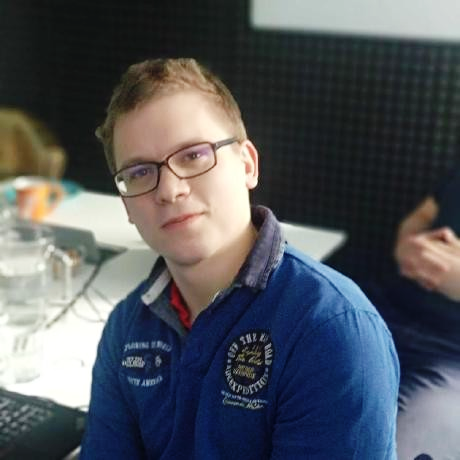
\includegraphics[scale=0.23]{dominik.png}
		}
		\hspace{10pt}
		\parbox[c][3cm][c]{0.32\textwidth}{
			\begin{center}
				\factbubble{\huge{\textcolor{sectcol}{\textbf{Ing.}}}\\\small{\textcolor{sectcol}{\textbf{FIT VUT}}}}{1}{maincol}{sectcol}{thirdcol}\\
				\textcolor{textcol}{\textbf{Brno University of Technologies}}
			\end{center}
		}
		\hspace{10pt}
		\parbox[c][3cm][c]{0.29\textwidth}{
			\textcolor{textcol}{ I am  enthusiatist for AI and computer vision developer always looking for new chalanges. }
		}
	}
	
	
	%----------------------------------------------------------------------------------------
	%	AREAS OF EXPERTISE
	%----------------------------------------------------------------------------------------
	
	%\cvsect{Areas of interest}{0.29}{thirdcol}{textcol}\\[4pt]
	\mbox{
		\parbox[t][60pt][c]{0.35\textwidth}{		
			% LANGUAGES
			\cvsect{Foreign languages}{0.49}{thirdcol}{textcol}\\[4pt]
			\icontext{Language}{12}{\colorbox{maincol}{English (B2)}}\\
			\icontext{Language}{12}{\colorbox{maincol}{Spanish (C1)}}\\
			\icontext{Language}{12}{\colorbox{maincol}{German (B1)}}\\
		}
		
		\begin{minipage}{0.05\textwidth}
			\begin{center}
				\begin{tikzpicture}
					\draw[draw=sectcol,dashed, opacity=0.5] (0,-5) -- (0,-1);
				\end{tikzpicture}
			\end{center}
		\end{minipage}
		
		\parbox[t][120pt][b]{0.45\textwidth}{
			\textcolor{thirdcol}{\hrule}
			\colorbox{thirdcol}{ {\cvsection{Areas of interest}{#4}}}
			\begin{piechart}{360}{2}{bgcol}{textcol}{sectcol}
				\slice{30}{Backend}{maincol}
				\slice{15}{Image processing}{thirdcol}
				\slice{35}{Machine learning}{fourthcol}
				\slice{20}{Frontend}{fifthcol}
								
			\end{piechart}\\
		}
				
		
		% PIE CHART	
				
	}
	\begin{center}
		\begin{tikzpicture}
			\draw[draw=sectcol,dashed, opacity=0.5] (4,0) -- (-4,0);
		\end{tikzpicture}
	\end{center}
	\vspace{0pt}
	
	% BAR CHART
	\cvsect{Languages and technology}{0.49}{thirdcol}{textcol}\\[4pt]
	\mbox{\hspace{-24pt}
		\begin{barchart}{10}{5.5}{sectcol}{textcol}{sectcol}{maincol}{secondcol}{thirdcol}
			\baritem{90}{Python}{0}{0}{80}
			\baritem{90}{React.js}{0}{0}{60}
			\baritem{75}{C/C++}{0}{0}{40}
			\baritem{75}{Docker}{0}{0}{60}
			\baritem{90}{Tensorflow}{0}{0}{80}
			\baritem{90}{Docker}{0}{0}{70}
			\baritem{75}{Ansible}{0}{0}{40}
			\baritem{75}{Selenium}{0}{0}{60}
			\baritem{75}{Git}{0}{0}{80}
		\end{barchart}
		\hspace{10pt}
		
		% TEXTBOX
		\parbox[b][130pt][c]{0.4\textwidth}{\textcolor{textcol}{I like to work in agile teams following IT development best practices like clean code, code reviews, testable code etc. allowing as to feel productive and make a positive impact. \\ \\ My biggest joy in programming is refactoring and removing old unused code.}}
	}
	
	\begin{center}
		\begin{tikzpicture}
			\draw[draw=sectcol,dashed, opacity=0.5] (4,0) -- (-4,0);
		\end{tikzpicture}
	\end{center}
		% \begin{center}
	% \mbox{
	% 		\parbox[b][2cm][c]{3cm}{
	% 			\textcolor{textcol}{I regularly use Meteor, Git and Webstorm for my dev projects.}
	% 		}\hspace{12pt}
	% 		\bubbles{6/Webstorm, 5/Git, 5/Sourcetree, 4/Linux, 3/Office}{\cvsection{Technologies}}		
	% 	}
	% 	\end{center}
	%---------------------------------------------------------------------------------------
	%	ACTIVITIES
	%----------------------------------------------------------------------------------------
		
	\vspace{0pt}
	\cvsect{Fungus app}{0.49}{thirdcol}{textcol}\\[20pt]
	\mbox{
				
		% FACT BUBBLE
		\parbox[b][3.5cm][c]{3.2cm}{
			\factbubble{\textcolor{sectcol}{\mbox{\nolinebreak{\textbf{500 000}} }}\\\small{\textcolor{sectcol}{\textbf{downloads}}}}{0.85}{maincol}{sectcol}{thirdcol}
			\textcolor{textcol}{\textbf{    Google Play}}
		}
		
		% TEXT BOX
		\parbox[b][3cm][c]{2.9cm}{
			\textcolor{textcol}{I founded computer vision start-up. We are developing an application that classifies mushroom species based on the image and other metadata. The team currently has 3 members. }
		}
		
		% SQUARE BARS
		\squares{25/1 request per second ,25/High availibility, 25/Advanced AI,25/10s of TB analyzed}{1}
	}
\end{minipage}
\begin{minipage}{0.05\textwidth}
	\begin{center}
		\begin{tikzpicture}
			\draw[draw=sectcol,dashed, opacity=0.5] (0,-12) -- (0,12);
		\end{tikzpicture}
	\end{center}
\end{minipage}
\begin{minipage}{0.4\textwidth}
	%---------------------------------------------------------------------------------------
	%	EXPERIENCE / EDUCATION
	%----------------------------------------------------------------------------------------
	\vspace{56pt}
	\cvsect{Experience and Education}{0.4}{thirdcol}{textcol}\\[16pt]
	
	\hspace{60pt}\mbox{\legend{Experience}{1.8cm}{maincol} \legend{Projects}{1.4cm}{secondcol} \legend{Education}{1.5cm}{thirdcol}}
	\vspace{-50pt}
	\begin{center}
		
		% TIMELINE
		\begin{cvtimeline}{2014}{2021}{21.6}%{\linewidth}
			
			
			
			\linevent{6/2014}{12/2014}{PHP Programmer}{}
			{Bestone Service}
			{maincol}{June 2014}
			
			\linevent{6/2015}{8/2015}{Hardware programmer}{}
			{Codasip}
			{maincol}{June 2015}
			
			\linevent{1/2015}{1/2017}{Bachelors's Degree}{}
			{BUT}
			{thirdcol}{May 2015}
			
			\linevent{11/2016}{12/2020}{Developer}{}
			{Mushroom Identification app}{secondcol}{March 2017}
			
			\linevent{5/2017}{6/2017}{Ing. Graduation}{}
			{BUT}{thirdcol}{May 2017}
			
			\linevent{10/2017}{1/2018}{Python programmer}{}
			{IXPERTA}{maincol}{August 2017}
			
			\linevent{3/2018}{2/2019}{AI Programmer}{}
			{IXPERTA}{maincol}{January 2018}
			    
			\linevent{2/2019}{6/2020}{Software Engineer}{}
			{Vacuumlabs}{maincol}{February 2019}    
			
			\linevent{12/2019}{12/2020}{Founder and Developer}{}
			{Fungus app}{secondcol}{March 2019}
			
			\linevent{6/2020}{12/2020}{Computer vision engineer}{}
			{SANEZOO}{maincol}{June 2020}
			     
		\end{cvtimeline}
		%\tiny @BUT = Brno University of Technology
	\end{center}
\end{minipage}

\newpage
\newcommand{\cvsecta}[1]{% The only parameter is the section text
	\vspace{\baselineskip} % Whitespace before the section title
	\colorbox{thirdcol}{\textcolor{white}{\MakeUppercase{\textbf{#1}}}}\\% Section title
}

\setlength{\LTpre}{0pt} % Remove default whitespace before longtable
\setlength{\LTpost}{0pt} % Remove default whitespace after longtable

\setlength{\tabcolsep}{0pt} % No spacing between table columns

% Environment to hold a new list of entries
\newenvironment{entrylist}{
	\begin{longtable}[H]{l l}
		}{ 
	\end{longtable}
}

\newcommand{\entry}[4]{% First argument for the leftmost date(s) text, second is for the bold entry heading, third is for the bold right-aligned entry qualifier and the fourth is for the entry description
	\parbox[t]{0.175\textwidth}{% 17.5% of the text width of the page
		\textcolor{thirdcol}{#1} % Leftmost entry date(s) text
		
				
	}%
	&\parbox[t]{0.825\textwidth}{% 82.5% of the text width of the page
		\textbf{\textcolor{thirdcol}{#2}}% Entry heading text
		\hfill% Horizontal whitespace
		{\footnotesize \textbf{\textcolor{thirdcol}{#3}}}\\% Right-aligned entry qualifier text
		\textcolor{thirdcol}{#4} % Entry description text
		}\\\\}
	
	% Command to output a separator slash between lists, e.g. '  /  '
	\newcommand{\slashsep}{\hspace{3mm}/\hspace{3mm}}
	
	\vfill
	
	\cvsect{Projects}{0.49}{thirdcol}{textcol}\\[20pt]
	% TODO add highlights, links
	\begin{entrylist}
		\entry
		{6/2020 -- Present}
		{Sanezoo Unity}
		{Sanezoo}
		{I was working on creating complex AI driven system for visual QA in industry. 
			My responsibility was creation and optimisation of the core component, that integrated our algorithms to a product deployable to the customers. 
			\\ 
			\texttt{C++}\slashsep
			\texttt{Tensorflow}
		}
		\entry
		{2/2019 -- present}
		{Fungus App}
		{My project}
		{I created a mobile app that identifies mushrooms based on
			image. It has more than 300,000 downloads now.
			\\ 
			\texttt{Python}\slashsep
			\texttt{React native}\slashsep
			\texttt{Tensorflow}}
		\entry
		{2/2019 -- 3/2020}
		{StockTwits.com}
		{Vacuumlabs, Stocktwits.com}
		{As a part of a four-member frontend team I was working on the development, maintenance
			and refactoring of a social network dedicated to the Stock Exchange. Apart from
			developing new features we significantly improved the code quality.  
			\\ 
			\texttt{React}}
		\entry
		{5/2018 -- 2/2019}
		{Industrial Vision startup}
		{Ixperta}
		{As a backend team, we were creating a new system of visual quality control in the
			industry. The system had to be highly reliable as the whole production line was stopped
			when an error occurred. I was responsible for the computer vision part; doing pre-sales
			experiments, and integrating and tweaking existing image processing algorithms.
			\\ 
			\texttt{Docker Swarm}\slashsep
			\texttt{Ansible}\slashsep
			\texttt{Microservices architecture}\slashsep
			\texttt{Tensorflow}\slashsep
			\texttt{Python}}
		\entry
		{12/2017 -- 4/2018}
		{Škoda Auto testing}
		{Ixperta, Škoda Auto}
		{I was leading a team of three engineers. We were responsible for creating a testing
			framework for a team of 20 manual testers to be able to create and manage test cases
			in a web UI. Real cars, car parts, simulators and the company web application were
			connected to our system.
			We were fully responsible for the design of the product, selected technologies and dev-
			ops. I was responsible for the communication with the customer and addressing their
			feedback to develop an application to match their needs. I also trained the manual
			testers and saved them many hours of the most monotonous work every day by
			allowing them to concentrate on more sophisticated test cases. 
			\\ 
			\texttt{Python}\slashsep
			\texttt{Selenium}\slashsep
			\texttt{PostgreSQL}\slashsep
			\texttt{Docker}
		}
		\entry
		{6/2017 -- 12/2017}
		{Screenix}
		{Ixperta, Agrofert}
		{We were a team of four engineers. We created a tool for checking sanctioned people
			and organizations to comply with Czech international business law. There are public
			lists of terrorists, authored by the UN, governments and ONGs, that are organized in
			many different ways, each providing quite limited information. We had to tackle the
			fuzzy nature of the problem as many sanctioned subjects used different pseudonyms;
			and information was uncertain, incomplete, and possibly faked by the checked
			business partners.
			\\ 
			\texttt{Python}\slashsep
			\texttt{Docker}
		}
	\end{entrylist}
	
	
	
	\vfill
	%============================================================================%
	%
	%
	%
	%	DOCUMENT END
	%
	%
	%
	%============================================================================%
\end{document}